

\subsubsection{深度学习方法用于动态物体分割}
\newpage
随着深度学习在越来越多的计算机视觉任务中表现出优异的性能,近年来也有不少研究将深度学习用于解决动态物体的分割问题。

在动态物体分割的研究中,许多学者使用了空间变换网络(Spatial Transformer Networks)~\cite{2015spatial}。这是因为动态物体分割的过程中涉及动态物体的识别,而同一类物体的大小、位置、姿态往往在不同图片中不尽相同,因此需要网络能抵抗这些因素的干扰,准确识别出物体,即网络的识别需要有空间不变性(spatially invariant)。而空间变换网络能以自监督学习的方式在网络内部对空间数据进行变换处理,使其具有空间不变性。该网络结构可作为一个模块嵌入到任何物体识别、检测、分割网络中,提高网络的性能。

由于动态物体分割本质上是将视频流中的动态物体识别、分离的过程,因此它可用深度学习中的注意力机制(attention)解决。近年来,出现了许多将注意力机制用于动态物体分割的研究工作,例如~\cite{2014multiple}用强化学习的方式训练循环神经网络(recurrent neural network, RNN),引入注意力机制使其输出图片中的多个物体。

目前,深度学习用于动态物体分割的研究工作往往需要预定义刚体的类型、运动模式或数量。将三维点云或光流作为输入,深度网络预测出动态物体的掩膜。Byranvan和Fox等人提出了SE3-Net~\cite{se3},能够从三维点云中将预先定义好的$n$个动态物体的6自由度位姿以$SE(3)$的形式预测出来。SE3-Net设计了一个编码-解码网络,使用卷积和反卷积预测每个动态物体的掩膜和6自由度位姿。其中,编码网络由两个并行的卷积和全连接网络构成,将输入的三维点云分别变换成隐变量和控制向量(control vector)。随后,将隐变量和控制向量拼接起来,由解码器(同样由两个并行的反卷积和全连接网络构成)输出稠密的物体掩膜和$SE(3)$变换参数。最后,用一个非线性变换层将三维点云、物体掩膜和$SE(3)$变换融合,生成动态物体的三维点云。

\begin{figure}[htbp]
	\centering
	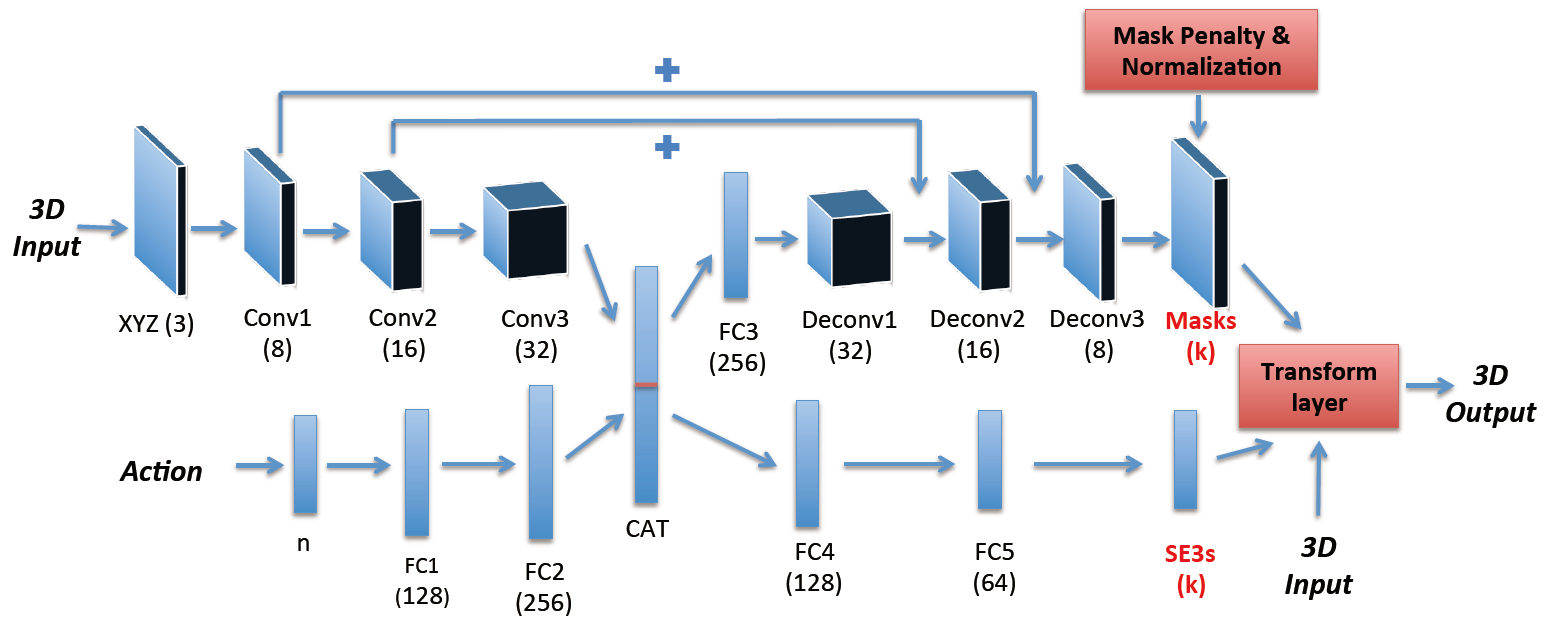
\includegraphics[width=0.9\textwidth]{figs/1-2/se3-net.png} 
	\label{se3-net}
	\caption{SE3-Net的网络结构图}
\end{figure}

Vijayanarasimhan等人通过实验证明,可以借助光流用深度学习分割场景中的动态物体~\cite{2017sfm}。他们设计了SfM-Net,通过显式的几何约束训练网络,使其可预测场景深度、相机运动和动态物体分割。SfM-Net由两个主流的卷积、反卷积网络构成,它们分别作为结构网络(structure network)和运动网络(motion network)。其中,结构网络通过学习预测场景深度,运动网络估计相机和物体位姿。在经过卷积网络的嵌入层(embedding layer)之后,通过两个全连接层输出动态物体的位姿估计。同时,嵌入层经过反卷积输出运动物体的掩膜估计。之后,通过估计的深度图,利用估计的相机和物体位姿将一帧RGB图像中的像素变换到另一帧的视角下,合成新视角下的图片,从而计算场景的光流。利用显示的几何约束关系,便可以自监督学习的方式通过最小化光度误差(photometric error)进行训练。

\begin{figure}[htbp]
	\centering
	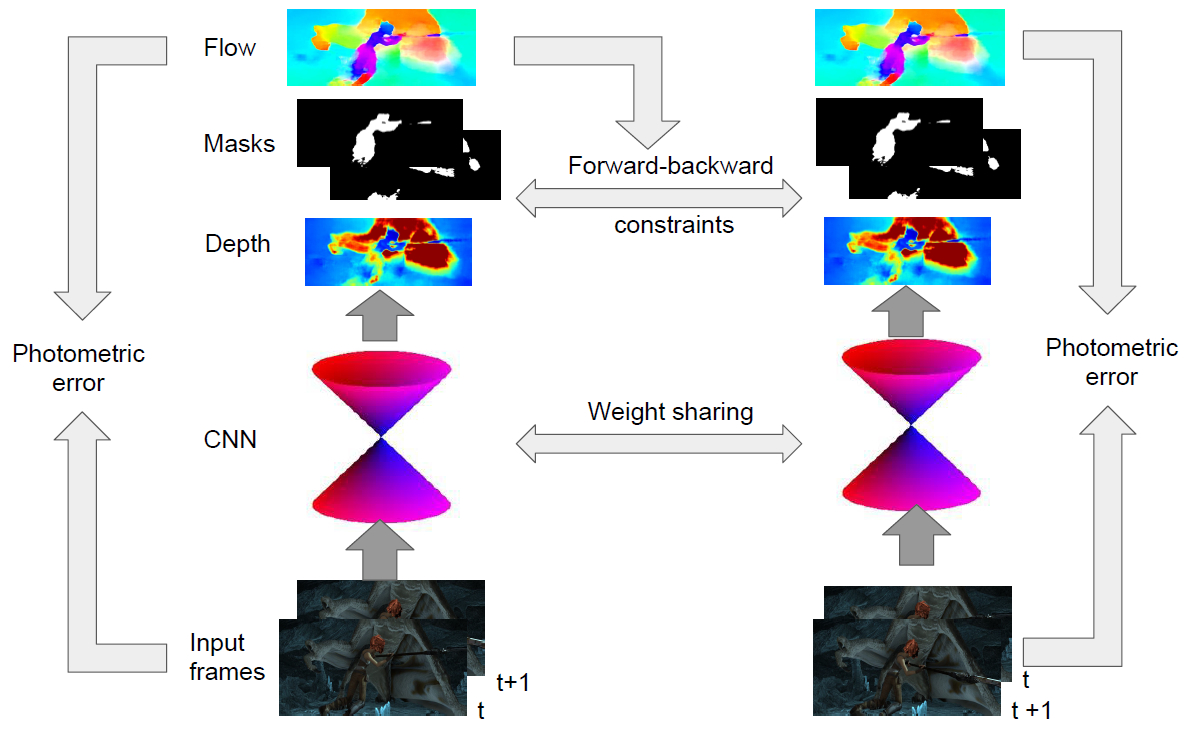
\includegraphics[width=0.7\textwidth]{figs/1-2/sfm-net.png} 
	\label{sfm-net}
	\caption{SfM-Net的流程图}
\end{figure}

\begin{figure}[htbp]
	\centering
	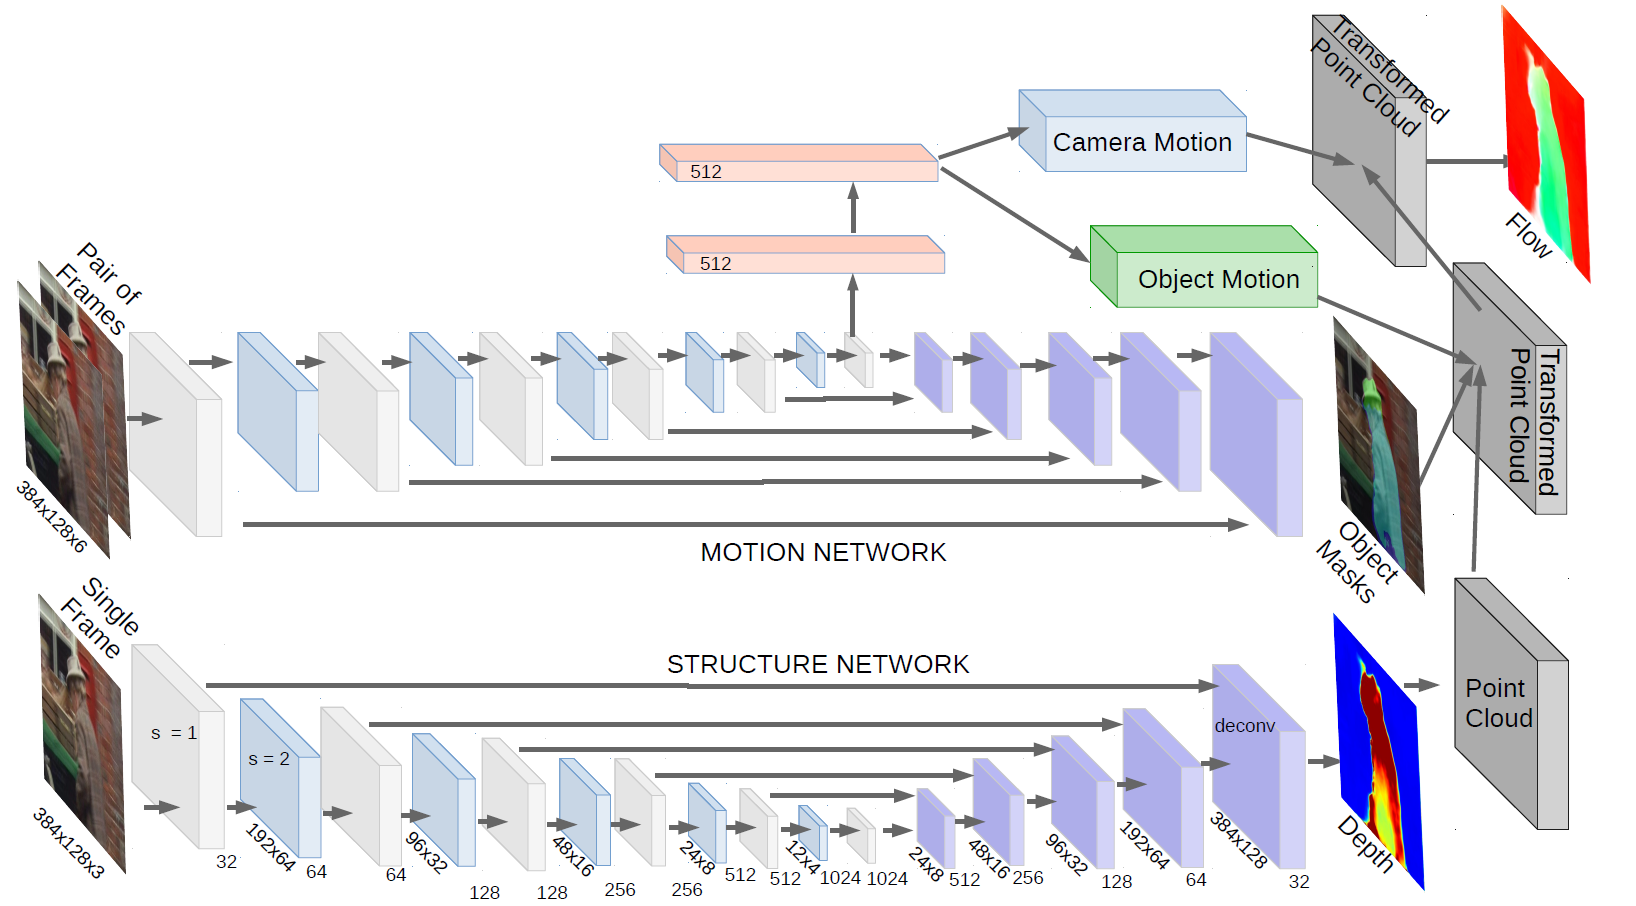
\includegraphics[width=0.9\textwidth]{figs/1-2/sfm-net2.png} 
	\label{sfm-net2}
	\caption{SfM-Net的网络结构图}
\end{figure}

与SfM-Net类似,Yin等人提出的GeoNet~\cite{geonet}自监督学习的方式,利用三维几何约束,将单目深度估计、光流估计和相机运动估计联合学习求解。为了能够恢复出完整场景的光流信息,GeoNet同样将场景显式地分为静态和动态部分,将各种估计通过视角合成生成新视角下的图片,并将损失函数建立在生成图片和拍摄图片的误差上,进行联合的自监督训练。如图~\ref{geonet},GeoNet利用前向和反向两个操作,判断区域内运动是由静态背景还是动态物体造成的,然后分别求解静态和动态部分的光流,合成整个场景的完整光流。另外,为增加对局外点(outlier)、光照变化、遮挡、无纹理和重复纹理区域的鲁棒性,GeoNet还使用了自适应的几何一致性损失函数。目前,GeoNet在室外车辆驾驶环境下,在深度、光流估计上均取得了非常不错的效果。

\begin{figure}[htbp]
	\centering
	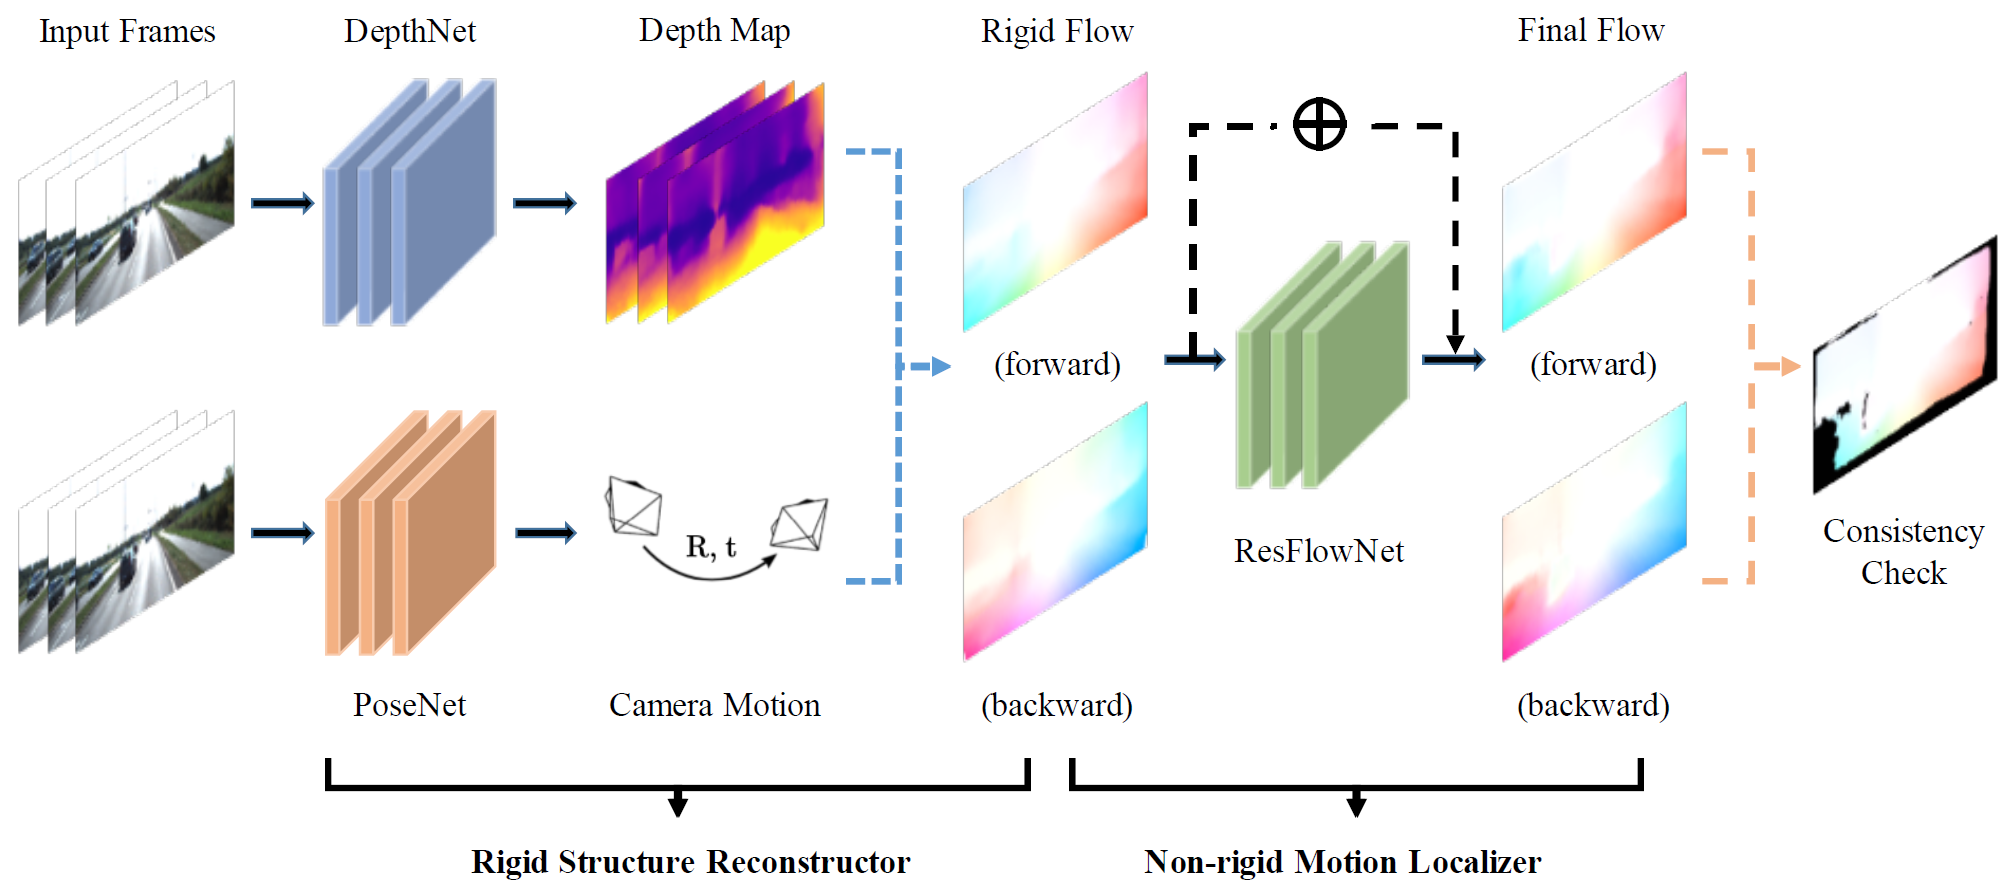
\includegraphics[width=0.9\textwidth]{figs/1-2/geonet.png} 
	\label{geonet}
	\caption{GeoNet的流程图}
\end{figure}

Lai等人认为,双目的深度估计和光流估计有其相同的地方,即寻找对应点的匹配和计算移动距离(视差),而此前的许多工作将二者分别用不同的网络估计,只在损失函数中将其耦合。因此,Lai等人将场景深度估计和光流估计用同一个网络求解~\cite{bridging},共享高维的特征表示,并在SfM-Net和GeoNet这类工作的思路下,充分利用了两个时刻双目图像之间的各种几何约束(如图~\ref{bridge}所示),使光流、深度估计的精度更高,从而有助于动态物体的分割。

\begin{figure}[htbp]
	\centering
	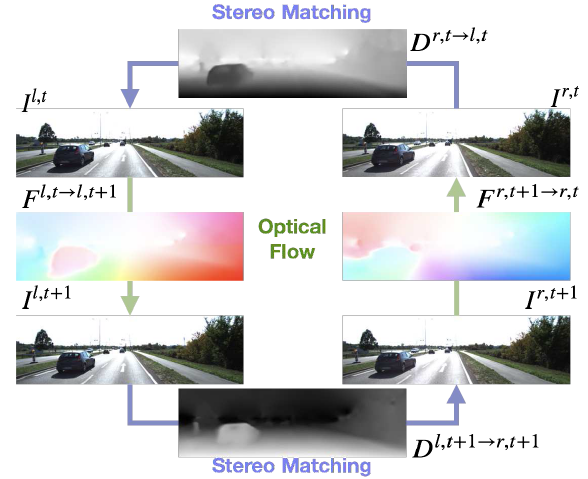
\includegraphics[width=0.43\textwidth]{figs/1-2/bridge1.png}
	\hspace{30pt}
	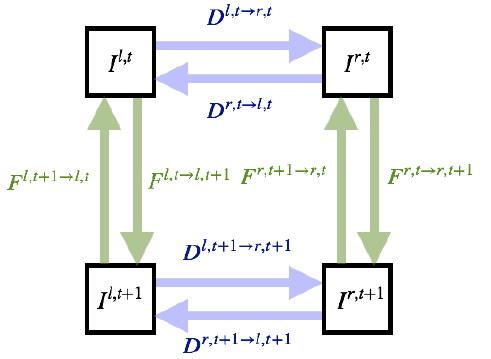
\includegraphics[width=0.43\textwidth]{figs/1-2/bridge2.png}
	\label{bridge}
	\caption{左边为~\cite{bridging}的流程图,右边为该方法利用的各种帧间几何约束}
\end{figure}

最近,Wang等人提出了UnOS网络,同样用双目自监督学习方法联合估计光流和场景深度~\cite{unos}。UnOS使用3个网络同时求解深度、相机位姿和刚性场景下的光流(rigid optical flow),并将刚性光流与FlowNet估计的光流作比较,找出符合刚性场景假设(rigid-scene assumption)即静态的部分。然后,促使两个光流估计在静态部分尽可能一致,那么余下的部分即是动态物体,由此得到动态物体的初步掩膜。之后,使用视觉里程计优化初步估计的掩膜,得到更精准的动态物体分割。在整个自监督训练过程中,除了图片合成作为损失函数之外,UnOS还使用了光流-深度一致性损失函数,使该方法在双目光流、深度估计、动态物体分割任务上均取得了很好的效果。

\begin{figure}[htbp]
	\centering
	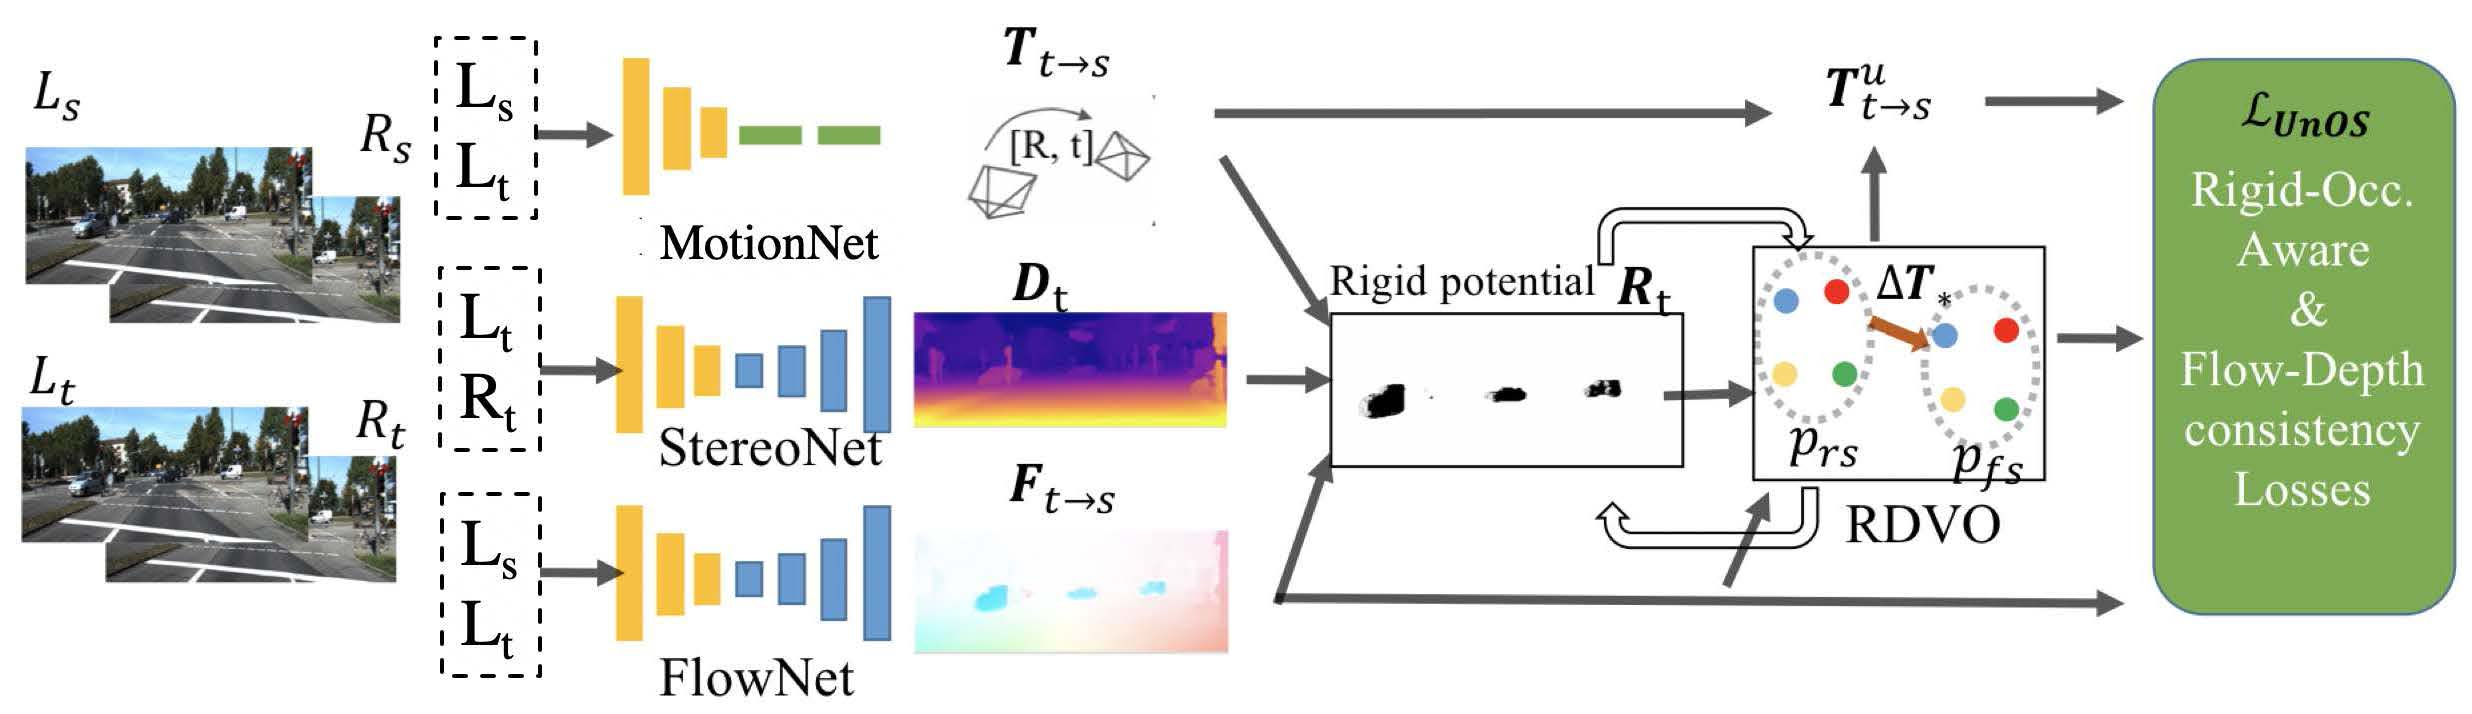
\includegraphics[width=0.9\textwidth]{figs/1-2/unos.jpg} 
	\label{geonet}
	\caption{UnOS的流程图}
\end{figure}


